\documentclass[10pt]{article}

\usepackage[spanish]{babel}
\usepackage[utf8]{inputenc}
\usepackage[T1]{fontenc}
\usepackage{lmodern}
\usepackage{siunitx}
\usepackage{amssymb}
\usepackage{csquotes}
\usepackage{float}
\usepackage{colortbl}
\usepackage{longtable}



\usepackage{booktabs} % Habilita \toprule, \midrule, \bottomrule y \addlinespace
\usepackage{tabularx} % Habilita el entorno tabularx y la columna dinámica 'X'
\usepackage{placeins} % Evita de forma estricta que las tablas cambien de sección

\usepackage[a4paper]{geometry}
\geometry{ margin=1.8cm
}

\usepackage{setspace}
\usepackage{amsmath}
\usepackage{graphicx}
\usepackage{pdfpages}
\usepackage{microtype}
\usepackage{xcolor}
\usepackage{titlesec}

\definecolor{formulaBlue}{RGB}{0,70,140}
\everymath{\color{formulaBlue}}
\everydisplay{\color{formulaBlue}}

\titleformat{\section} {\large\bfseries} {\thesection} {1em} {}

\setlength{\parskip}{2pt}

\renewcommand{\contentsname}{Índice}

\usepackage[colorlinks=true, linkcolor=black, citecolor=black, urlcolor=blue, hypertexnames=false]{hyperref}

\usepackage[backend=biber,style=authoryear]{biblatex}

% Separación autor-año en las citas parentéticas
\renewcommand*{\nameyeardelim}{\addcomma\space}

\addbibresource{referencias.bib}


\title{Finanzas Largo Plazo 2026 Volumen 6}
\author{
Roger Román Armoa García\\
\small
ORCID: \href{https://orcid.org/0009-0008-9149-3619}
{0009-0008-9149-3619}
}
\date{Asunción -- 2026}


\setlength{\abovedisplayskip}{6pt}
\setlength{\belowdisplayskip}{6pt}
\setlength{\abovedisplayshortskip}{4pt}
\setlength{\belowdisplayshortskip}{4pt}

\usepackage{tcolorbox}

\newtcolorbox{intuicion}{ colback=blue!5!white, colframe=blue!75!black, title=Intuición
}

\newtcolorbox{resumen}{ colback=gray!10!white, colframe=black!75!white, title=Resumen del Flujo Económico
}

\newtcolorbox{formula}{ colback=blue!5!white, colframe=formulaBlue, title=Fórmula Clave, fontupper=\everymath{\color{black}}\everydisplay{\color{black}}
}

\newtcolorbox{error}{ colback=red!5!white, colframe=red!75!black, title=¡Cuidado! Error Común
}

\usepackage{pifont}
\DeclareUnicodeCharacter{2714}{\ding{51}}

% Colores para tablas y calendarios
\usepackage{xcolor}
\usepackage{colortbl}

\definecolor{calAzul}{HTML}{17365D}
\definecolor{calAzulClaro}{HTML}{DCE6F1}
\definecolor{calVerdeClaro}{HTML}{E2F0D9}
\definecolor{calAmarilloClaro}{HTML}{FFF2CC}
\definecolor{calGrisClaro}{HTML}{F2F2F2}

\begin{document}

\pagenumbering{gobble}
\thispagestyle{empty}

\begin{center}
\vspace*{\fill}
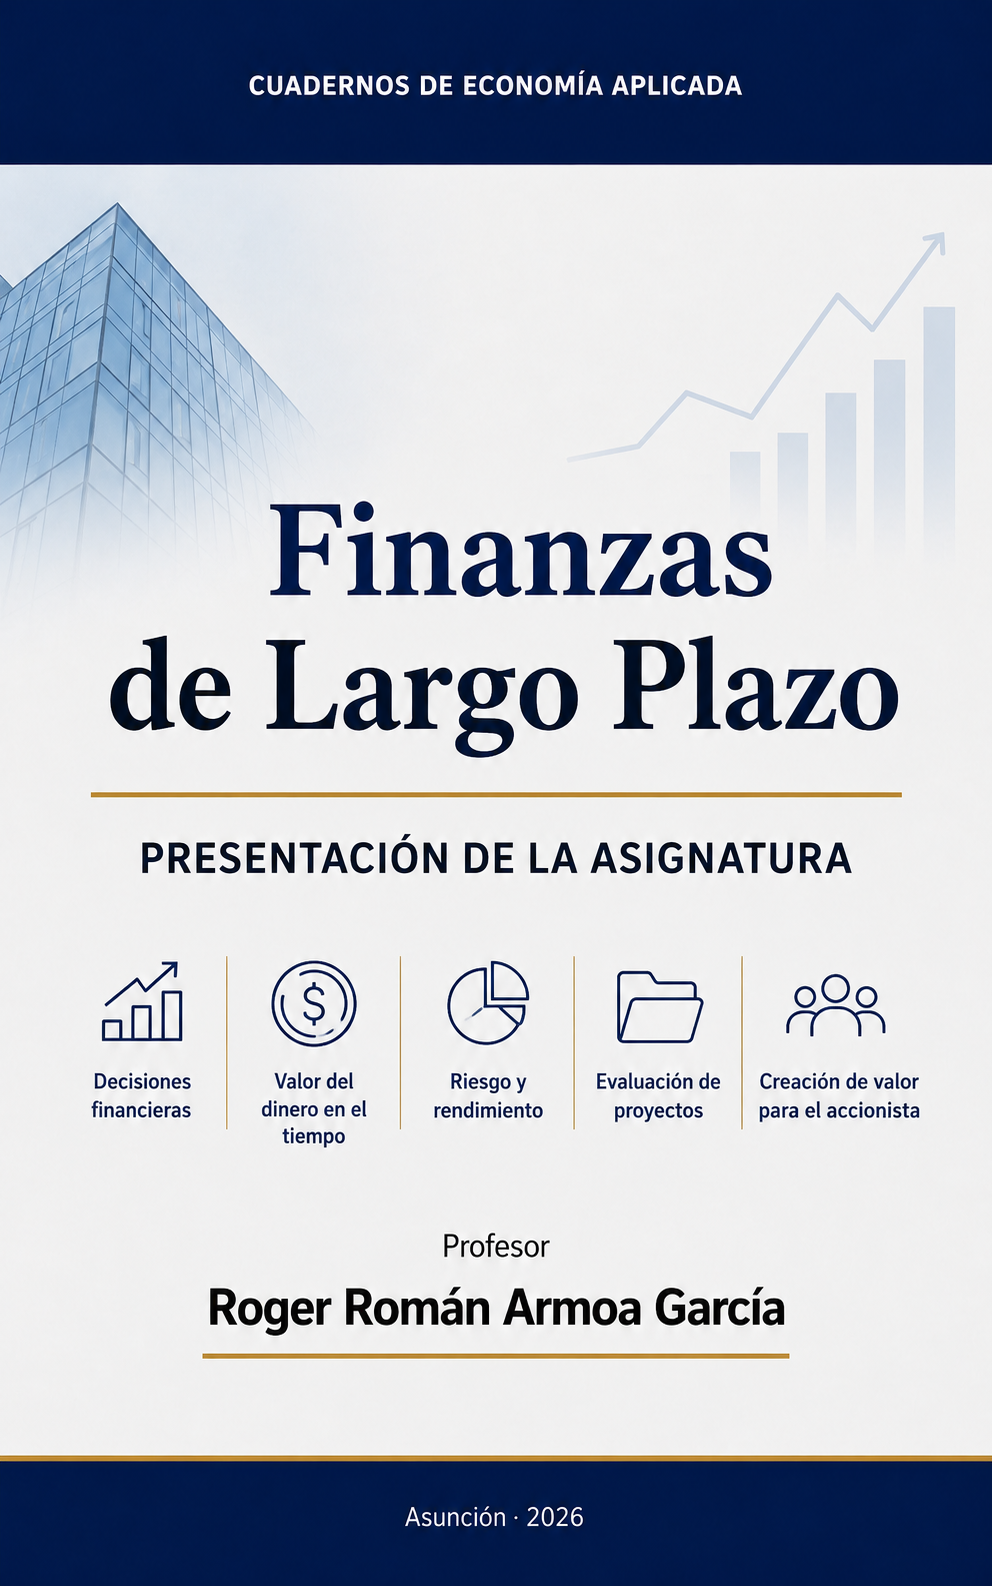
\includegraphics[width=0.8\paperwidth,height=0.8\textheight,keepaspectratio]{portada_presentacion_asignatura_v1.png}
\vspace*{\fill}
\end{center}

\clearpage
\maketitle

\section*{Colección}
\addcontentsline{toc}{section}{Colección}

\textbf{Cuadernos de Finanzas Largo Plazo}

Universidad Americana  \\ Campus Asunción \\ Facultad de Ciencias Económicas y Administrativas \\
Carrera de Economía \\ Grupo 80 -- Presencial

Editor académico: Roger Román Armoa García

Esta colección simplifica el estudio de la asignatura en Modelo de Aprendizaje Basado en Competencias (MAC).\parencite{uaModeloCompetencias}
\newpage

\section*{Página legal}
\addcontentsline{toc}{section}{Página legal}

\textbf{Finanzas Largo Plazo 2026}

Colección: Cuadernos de Finanzas Largo Plazo\\
Volumen 6

\begin{flushleft}
    \textbf{Volumen 6} \\[0.5em]
    
\textbf{Autor:} \\
Roger Román Armoa García \\

\textbf{ORCID:}
\href{https://orcid.org/0009-0008-9149-3619}
{0009-0008-9149-3619}
\\[1em]

    
    \textbf{Filiación institucional:} \\
    Universidad Americana \\
    Facultad de Ciencias Económicas y Administrativas \\[1em]

    \textbf{Carrera:} \\
    Economía \\[1em]

    \textbf{Grupo y modalidad:} \\
    Grupo 80 -- Presencial
\end{flushleft}



Asignatura: Finanzas a Largo Plazo\\
Código de la asignatura: ECO-132

Asunción, Paraguay\\
Primera edición: 2026

\bigskip

© 2026 Roger Román Armoa García
\\ Clasificación Decimal Dewey: 658.15
\vfill

\begin{center}
{\small ISBN: pendiente de asignación}
\vspace{0.3cm}
% \includegraphics[width=0.45\textwidth]{isbn_978-99989-1-850-4.png}
\end{center}

\clearpage
\tableofcontents
\cleardoublepage

\pagenumbering{arabic}
\setcounter{page}{1}

\begin{tcolorbox}[
colback=gray!5,
colframe=black,
title=\textbf{Datos de identificación del trabajo},
sharp corners,
boxrule=0.8pt,
width=\textwidth
]

\renewcommand{\arraystretch}{1.8}

\begin{tabular}{p{0.24\textwidth} p{0.70\textwidth}}

\textbf{Nombre y apellido:} & \hrulefill \\

\textbf{Asignatura:} &
Finanzas a Largo Plazo \\

\textbf{Carrera:} &
Economía \\

\textbf{Facultad:} &
Facultad de Ciencias Económicas y Administrativas \\

\textbf{Universidad:} &
Universidad Americana \\

\textbf{Grupo/Sección:} &
Grupo 80 -- Presencial \\

\textbf{Docente:} &
Roger Román Armoa García \\

\textbf{Fecha:} &
\hrulefill \\

\end{tabular}

\end{tcolorbox}

\section{Introducción al enfoque de enseñanza por competencias}

\subsection{Enfoque general de la asignatura}

En este enfoque de enseñanza el profesor asume el papel de guía del aprendizaje y es el alumno quien construye los conocimientos y muestra evidencias de que adquiere la competencia. Por esta razón, uno de los primeros puntos que definimos con los alumnos es la competencia que queremos lograr en la asignatura, luego en la unidad y, por último, en la clase.\parencite{uaModeloCompetencias,armoa2026planeamiento}

\subsection{Evidencias de aprendizaje}

Mi propuesta para que muestren evidencias de que adquieren la competencia que buscamos consiste en la elaboración y presentación de un PDF. Por esta razón, una de las primeras asignaciones consiste en que cada uno elabore informes en formato PDF con la herramienta de software que prefiera.

El profesor realiza correcciones sucesivas sobre este trabajo hasta llegar al formato que queremos obtener en el documento final.

De manera general, el proceso consiste en:

\begin{itemize}
    \item elaborar una primera versión del PDF;
    \item presentar el trabajo para su revisión;
    \item recibir observaciones y correcciones;
    \item realizar los ajustes necesarios;
    \item presentar nuevas versiones hasta alcanzar el formato esperado.
\end{itemize}

\begin{figure}[H]
    \centering
    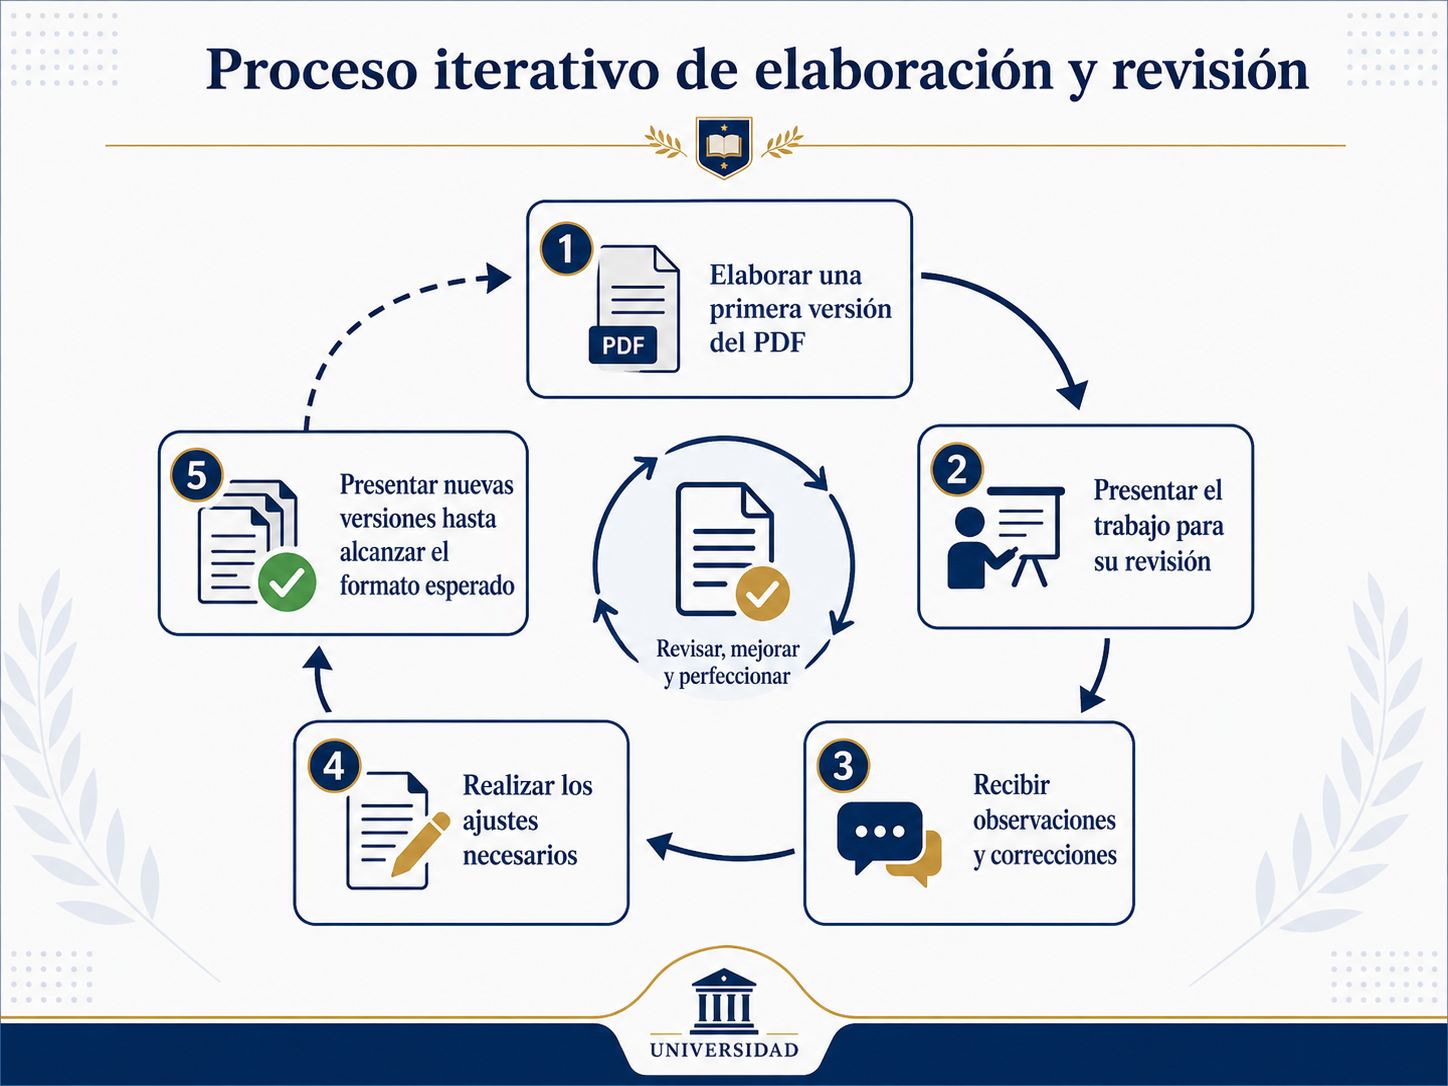
\includegraphics[width=0.50\textwidth]{proceso_iterativo.png}
    \caption{Proceso iterativo de elaboración y revisión del material.}
    \label{fig:proceso_iterativo}
\end{figure}


\subsection{Presentación e integración del grupo}

También me interesa conocerlos personalmente, ya que nuestra modalidad es presencial. Por eso, les pido que completen el formulario de datos personales y que se acerquen a mí para conversar brevemente.

También podemos realizar una presentación ante todo el grupo. El objetivo es que yo los conozca y que ustedes se conozcan entre sí. Es una actividad para romper el hielo que parece trivial, pero es importante para facilitar el trabajo conjunto durante el semestre.

Este grupo corresponde a la carrera de \textbf{Economía}, Grupo 80, modalidad presencial. La asignatura asignada al grupo se identifica con el código \textbf{ECO-132}. La existencia de asignaturas con denominaciones similares en otras carreras no implica, por sí sola, que correspondan al mismo código, programa o grupo.

\subsection{Propósito de la primera actividad}

No los subestimo al pedirles que preparen un PDF. Es muy probable que ustedes ya manejen estas herramientas mejor que estudiantes de promociones anteriores, por así decirlo. Sin embargo, con frecuencia encuentro dificultades que son muy comunes al elaborar un informe, y me interesa que nos preparemos bien en este aspecto para evitar esos mismos problemas.

\subsection{Clases en Aula}

Por su carácter aplicado, la asignatura contempla actividades prácticas en aula. Para estas actividades se utilizan recursos informáticos asignados institucionalmente, de acuerdo con su disponibilidad y con la planificación correspondiente a cada clase.\parencite{armoa2026planeamiento}

En las aulas no contamos con ordenadores, pero sí contamos con Wi-Fi, además de recursos para presentación y conectividad para el profesor. Cuando el acceso a los equipos requiere credenciales, estas son proporcionadas conforme a los procedimientos definidos por los responsables de la sala.

Las actividades de laboratorio se articulan con la metodología de construcción de clases adoptada en la asignatura. El docente presenta una orientación inicial y los estudiantes desarrollan las tareas prácticas, recopilan y contrastan información, construyen evidencias de aprendizaje y aportan los resultados obtenidos a la base de conocimientos que se discute y valida durante la clase.

Para facilitar la coordinación previa y posterior a los encuentros presenciales, se utiliza un canal de mensajería instantánea definido para el grupo. Durante el periodo académico 2026 se propone el uso de WhatsApp como medio complementario de comunicación para informar el lugar de inicio de la clase, los laboratorios asignados y otras cuestiones operativas relacionadas con el desarrollo de las actividades.

Este canal complementa, pero no sustituye, los medios académicos e institucionales que correspondan. Su utilización facilita especialmente la coordinación de las actividades que se desarrollan fuera del aula o del laboratorio, dado que la carga académica de la asignatura incluye tanto trabajo con acompañamiento docente como trabajo independiente.

\subsection{Medición de la competencia adquirida}

La adquisición de competencias requiere un proceso de medición que permita comparar los resultados alcanzados con la situación inicial de los estudiantes. Esta medición se considera en tres niveles: asignatura, unidad didáctica y clase.

Por razones de practicidad, en esta primera experiencia proponemos realizar una medición diagnóstica y formativa inicial a nivel general de la asignatura. Su propósito es disponer de un punto de referencia que permita reconocer los conocimientos y competencias que los estudiantes poseen al comienzo del periodo académico y, posteriormente, contrastarlos con los resultados que alcanzan durante el desarrollo de la asignatura.\parencite{armoa2026planeamiento}

Además de identificar el nivel inicial de competencias, resulta importante conocer los intereses académicos y profesionales de los estudiantes. Por esta razón, el instrumento inicial puede incorporar información sobre las áreas de interés de cada participante. La lectura de estas respuestas permite obtener, desde la primera clase, una aproximación al nivel de conocimientos del grupo y a sus principales ámbitos de interés.

Esta información contribuye a orientar las actividades de aprendizaje y a evitar, en la medida de lo posible, una dedicación innecesaria de tiempo a contenidos que el grupo ya domina. El tiempo disponible para la asignatura constituye un recurso limitado y, por ello, se procura destinarlo prioritariamente a actividades que aporten valor al aprendizaje y que resulten útiles a corto, mediano y largo plazo.

La medición inicial se integra con la metodología de construcción de clases adoptada en la asignatura. A partir del diagnóstico, el docente presenta una estructura inicial de temas y subtemas, mientras que los estudiantes construyen y amplían la base de conocimientos, incorporan información a la matriz de trabajo y participan en la discusión y validación de los contenidos desarrollados.

\subsubsection{Registro de asistencia}

La asignatura requiere también un registro sistemático de la asistencia presencial. Debido a que este grupo aplica este requisito de manera especialmente rigurosa, se establece inicialmente un procedimiento operativo que puede ser revisado y perfeccionado a medida que se evalúa su funcionamiento.

\subsection{Medios digitales}

Para el registro de las evidencias de participación que habitualmente se consignan mediante la firma del docente en el cuaderno, los estudiantes pueden utilizar también dispositivos digitales, como tabletas.

Cuando el dispositivo dispone de un lápiz digital que permite incorporar escritura manuscrita, el docente puede realizar la firma directamente sobre el documento o archivo correspondiente. En estos casos, el estudiante es responsable de conservar adecuadamente el registro digital y de mantener copias de respaldo que permitan preservar las evidencias de participación durante todo el periodo académico.

El uso de medios digitales no modifica la finalidad del registro: documentar la participación del estudiante y conservar evidencias de su proceso de aprendizaje. Estos registros complementan las evidencias generadas mediante la metodología de construcción de clases, en la que los estudiantes desarrollan, documentan y consolidan progresivamente los conocimientos trabajados durante cada encuentro.

Como alternativa, cuando el estudiante utiliza este mismo documento en formato PDF y dispone de un dispositivo que permite escritura manuscrita digital, el docente puede incorporar la firma directamente en la ficha de identificación ubicada al inicio del documento o en el espacio destinado al registro de participación. De este modo, el propio PDF puede conservar las evidencias de participación correspondientes a la asignatura, siempre que el estudiante mantenga una copia íntegra, actualizada y debidamente respaldada del archivo.


\section{Programa de estudios y competencias}

El programa rector vigente para esta asignatura corresponde a
\textbf{Finanzas a Largo Plazo -- ECO-132}, carrera de Economía, Grupo 80,
modalidad presencial. El programa establece una carga horaria total de
\textbf{51 horas}, distribuidas en \textbf{15 horas teóricas} y
\textbf{36 horas prácticas}, y organiza los contenidos curriculares en
\textbf{cuatro unidades}.
\parencite{uaProgramaFinanzasLargoPlazo}

El objetivo general consignado en el programa es:

\begin{quote}
Aplicar los conocimientos sobre la estructura económica y financiera
organizacional que analizan las inversiones a largo plazo, para la toma de
decisiones de tipo económico a través de diferentes herramientas o modelos
que le garanticen la permanencia en el entorno y en el tiempo.
\end{quote}
\parencite{uaProgramaFinanzasLargoPlazo}

El programa ECO-132 recibido no explicita objetivos específicos diferenciados
por unidad. Por esta razón, las competencias de unidad que se presentan a
continuación constituyen una formulación didáctica derivada del objetivo general
y de los contenidos curriculares, destinada a expresar desempeños observables
del estudiante. El planeamiento de cátedra concreta estos contenidos mediante
resultados de aprendizaje, actividades, evidencias e instrumentos de evaluación.
\parencite{armoa2026planeamiento}

\subsection{Presentación e indagación inicial}

Antes del desarrollo de las unidades temáticas se realiza una instancia de
presentación e indagación inicial. En ella se presentan los objetivos de la
asignatura, la metodología de trabajo, los criterios de evaluación, las normas
generales, los recursos disponibles y el uso de las plataformas digitales.
\parencite{armoa2026planeamiento}

Esta instancia permite identificar los conocimientos previos y los intereses
académicos y profesionales de los estudiantes. La información obtenida
constituye una referencia inicial para orientar las clases y posteriormente
contrastar la evolución del aprendizaje.

\textbf{Propósito de la instancia inicial:} identificar las condiciones de
partida del estudiante y asegurar que comprenda la organización, metodología
y criterios generales de funcionamiento de la asignatura.

\subsection{Unidad I. Introducción a las Finanzas Empresariales}

El programa ECO-132 establece para esta unidad los siguientes contenidos:
\textit{Síntesis de la Administración Financiera; el entorno financiero:
mercados, instituciones y tasas de interés; lectura de Estados Financieros
Internacionales y Paraguayos; y objetivo básico financiero}.
\parencite{uaProgramaFinanzasLargoPlazo}

\textbf{Competencia de la unidad:} interpretar el papel de la administración
financiera, el entorno financiero y la información contenida en los estados
financieros, relacionándolos con el objetivo básico financiero y con la toma de
decisiones empresariales.

\paragraph{Lecturas para el estudio de la unidad.}

\textbf{Van Horne y Wachowicz (2010), \textit{Fundamentos de Administración
Financiera}, 13.ª edición:}

\begin{itemize}
    \item Capítulo 1, \textit{El papel de la administración financiera},
    pp.~1--14: administración financiera, meta de la compañía y función
    financiera en la organización.
    \item Capítulo 2, \textit{Entornos de negocios, fiscales y financieros},
    pp.~17--39: entorno de negocios, entorno fiscal y entorno financiero.
    \item Capítulo 6, \textit{Análisis de estados financieros},
    pp.~127--167: estados financieros, marco de análisis, razones financieras,
    tendencias y análisis de tamaño común.
\end{itemize}
\parencite{vanhorne2010fundamentos}

\noindent
La lectura se complementará con estados financieros internacionales y
paraguayos seleccionados para la clase y con la bibliografía básica establecida
en el programa ECO-132.

\subsection{Unidad II. Estructura de Capital, Fuentes de Financiamiento y Costo de Capital}

El programa contempla conceptos de estructura de capital, antecedentes del
costo de capital, costos de las diferentes fuentes de financiamiento, costo de
la deuda y del capital, WACC, CAPM, beta apalancada y no apalancada, y las
decisiones de estructura de capital relacionadas con la maximización de la
riqueza de los accionistas.
\parencite{uaProgramaFinanzasLargoPlazo}

\textbf{Competencia de la unidad:} calcular y analizar el costo de las fuentes
de financiamiento, CAPM, beta y WACC, y utilizar esos resultados para comparar
alternativas de estructura de capital y fundamentar decisiones orientadas a la
creación de valor.

\paragraph{Lecturas para el estudio de la unidad.}

\textbf{Van Horne y Wachowicz (2010), 13.ª edición:}

\begin{itemize}
    \item Capítulo 5, \textit{Riesgo y rendimiento}, pp.~97--116:
    riesgo, rendimiento y fundamentos del CAPM.
    \item Capítulo 15, \textit{Rendimientos requeridos y costo de capital},
    pp.~381--406: costo de las fuentes de financiamiento, rendimiento requerido
    y costo promedio ponderado de capital. Como ampliación, los apéndices del
    capítulo se encuentran en pp.~407--418.
    \item Capítulo 17, \textit{Determinación de la estructura de capital},
    pp.~451--474: estructura de capital, valor, impuestos, señales y criterios
    de financiamiento.
\end{itemize}

\textbf{Brigham y Houston (2020), 15.ª edición:}
\begin{itemize}
    \item Capítulo 10, \textit{El costo del capital}, pp.~356--384.
    \item Capítulo 14, \textit{Estructura de capital y apalancamiento},
    pp.~474--516.
\end{itemize}

\textbf{Material aplicado de la asignatura:}
\textit{Conceptos fundamentales de finanzas de largo plazo}, vol.~1,
pp.~1--14, y \textit{Finanzas de largo plazo: Ejercicios}, vol.~2,
pp.~2--19, para ejercicios de CAPM y WACC.
\parencite{vanhorne2010fundamentos,brigham2020fundamentos,armoa2026conceptos,armoa2026ejercicios}

\subsection{Unidad III. Análisis de Inversiones}

El programa ECO-132 comprende flujo de caja del inversionista y del proyecto;
indicadores económicos y financieros ---VAN, TIR, Payback e Índice de
Rentabilidad---; análisis de sensibilidad; EBITDA y su importancia en las
finanzas de la empresa; y la relación entre estados financieros y EVA.
\parencite{uaProgramaFinanzasLargoPlazo}

\textbf{Competencia de la unidad:} construir y analizar flujos de caja de
proyectos e inversionistas, aplicar indicadores de evaluación de inversiones y
análisis de sensibilidad, e interpretar EBITDA y EVA para fundamentar una
decisión económica.

\paragraph{Lecturas para el estudio de la unidad.}

\textbf{Van Horne y Wachowicz (2010), 13.ª edición:}
\begin{itemize}
    \item Capítulo 7, \textit{Análisis de fondos, análisis de flujo de efectivo
y planeación financiera}, pp.~169--203.
    \item Capítulo 12, \textit{Presupuesto de capital y estimación de los
flujos de efectivo}, pp.~307--322.
    \item Capítulo 13, \textit{Técnicas para elaborar el presupuesto de
    capital}, pp.~323--340: Payback, TIR, VAN e índice de rentabilidad. Como
    ampliación, los apéndices del capítulo se encuentran en pp.~341--352.
    \item Capítulo 14, \textit{Riesgo y opciones administrativas (reales) de
    presupuesto de capital}, pp.~353--380, como apoyo al análisis de riesgo y
    sensibilidad.
\end{itemize}

\textbf{Brigham y Houston (2020), 15.ª edición:}
\begin{itemize}
    \item Capítulo 11, \textit{Elementos de la presupuestación del capital},
    pp.~385--416.
    \item Capítulo 12, \textit{Estimación de flujos de efectivo y análisis de
riesgo}, pp.~417--452.
\end{itemize}

\textbf{Material aplicado de la asignatura:}
\textit{Finanzas de largo plazo: Ejercicios}, vol.~2, pp.~2--29, para
indicadores, flujo de fondos y evaluación de proyectos.
\parencite{vanhorne2010fundamentos,brigham2020fundamentos,armoa2026ejercicios}

\noindent
Los contenidos específicos de EBITDA y EVA se trabajarán además con la
bibliografía básica oficial del programa ECO-132 y con estados financieros
seleccionados. No se consignan páginas adicionales hasta fijar y verificar la
edición concreta utilizada para esos apartados.

\subsection{Unidad IV. Estructuras Financieras Óptimas}

La cuarta unidad comprende enfoques tradicionalistas y de Modigliani--Miller,
capacidad de endeudamiento de la empresa, comparaciones y decisiones de
financiamiento, análisis del ROE, análisis del modelo UAII/GPA y política de
dividendos en relación con la estructura financiera.
\parencite{uaProgramaFinanzasLargoPlazo}

\textbf{Competencia de la unidad:} comparar estructuras financieras y
alternativas de financiamiento mediante criterios de endeudamiento,
apalancamiento, ROE, UAII/GPA y política de dividendos, fundamentando una
recomendación coherente con la creación de valor.

\paragraph{Lecturas para el estudio de la unidad.}

\textbf{Van Horne y Wachowicz (2010), 13.ª edición:}
\begin{itemize}
    \item Capítulo 16, \textit{Apalancamiento financiero y operativo},
    pp.~419--450: apalancamiento, riesgo financiero y capacidad de la empresa
    para atender compromisos derivados del financiamiento.
    \item Capítulo 17, \textit{Determinación de la estructura de capital},
    pp.~451--474: enfoques de estructura de capital y decisiones de
    financiamiento.
    \item Capítulo 18, \textit{Política de dividendos}, pp.~475--504.
\end{itemize}

\textbf{Brigham y Houston (2020), 15.ª edición:}
\begin{itemize}
    \item Capítulo 14, \textit{Estructura de capital y apalancamiento},
    pp.~474--516.
    \item Capítulo 15, \textit{Distribuciones a los accionistas: dividendos y
    recompras de acciones}, pp.~517--550.
\end{itemize}

\textbf{Material aplicado de la asignatura:}
\begin{itemize}
    \item \textit{Finanzas de largo plazo: Arbitraje de acciones}, vol.~4,
    pp.~1--18, para apalancamiento, arbitraje, UAII/GPA y alternativas de
    financiamiento.
    \item \textit{Finanzas de largo plazo: Política de dividendos}, vol.~5,
    pp.~1--22, para política de dividendos, señales, agencia y recompras.
\end{itemize}
\parencite{vanhorne2010fundamentos,brigham2020fundamentos,armoa2026arbitraje,armoa2026dividendos}

\subsection{Articulación de las competencias}

Las cuatro unidades conforman un recorrido progresivo. La primera establece
la función de la administración financiera, el entorno y la lectura de la
información financiera. La segunda desarrolla las fuentes de financiamiento,
el costo de capital y las decisiones de estructura de capital. La tercera
traslada esos fundamentos al análisis de inversiones mediante flujos,
indicadores, sensibilidad, EBITDA y EVA. La cuarta integra las decisiones de
financiamiento mediante estructuras financieras óptimas, capacidad de
endeudamiento, ROE, UAII/GPA y política de dividendos.
\parencite{uaProgramaFinanzasLargoPlazo,armoa2026planeamiento}

El énfasis de la asignatura es aplicado: los estudiantes utilizan herramientas
computacionales, particularmente planillas de cálculo, verifican la coherencia
de los datos, ejecutan los procedimientos cuantitativos, interpretan resultados
y fundamentan decisiones financieras.

\section{Comentarios sobre la bibliografía y el uso de NotebookLM}

En esta asignatura se utilizan herramientas de inteligencia artificial (IA) como apoyo al aprendizaje. Estas herramientas pueden facilitar la búsqueda, organización, análisis y síntesis de información, pero no sustituyen la responsabilidad académica del estudiante ni la necesidad de verificar las fuentes utilizadas.

Para el periodo académico 2026 se recomienda el uso de NotebookLM, una herramienta de Google disponible en:\parencite{googleNotebookLM}

\begin{center}
\url{https://notebooklm.google.com/}
\end{center}

NotebookLM permite trabajar con fuentes seleccionadas previamente por el usuario. A partir de esos documentos, es posible realizar consultas, obtener resúmenes, comparar información y generar explicaciones basadas en el material proporcionado.\parencite{googleNotebookLM}

Cuando exista disponibilidad institucional, los estudiantes podrán utilizar NotebookLM mediante las cuentas y equipos habilitados por la Facultad. Las condiciones de acceso pueden depender de las políticas institucionales y de las condiciones establecidas por el proveedor.


\subsection{Selección y control de las fuentes}

Las herramientas de inteligencia artificial pueden ayudar a buscar, organizar y explicar información. Sin embargo, una respuesta generada por una herramienta de IA no necesariamente es correcta. La calidad de la respuesta depende, en buena medida, de la calidad de la información utilizada como fuente.

Por esta razón, en la asignatura se dará especial importancia a trabajar con fuentes confiables. Se utilizarán principalmente libros, artículos científicos, documentos técnicos, publicaciones oficiales y otros materiales cuya procedencia pueda ser verificada.

NotebookLM facilita este trabajo porque permite seleccionar previamente los documentos que se utilizarán como fuentes. El estudiante puede realizar preguntas sobre esos documentos y luego comprobar si las respuestas obtenidas están realmente respaldadas por ellos.\parencite{googleNotebookLM}

El uso de inteligencia artificial no reemplaza la revisión del estudiante. Siempre será necesario comprobar la información, interpretar correctamente los resultados y verificar que las afirmaciones realizadas estén sustentadas por las fuentes utilizadas.

Como referencia principal para el estudio de la asignatura, se recomienda especialmente el libro de \textcite{vanhorne2010fundamentos}.

\subsection{Procedimientos de revisión de respuestas generadas por IA}

Durante la asignatura se emplean también procedimientos destinados a aumentar el nivel de revisión crítica de las respuestas obtenidas mediante herramientas de inteligencia artificial.

Entre estos procedimientos se encuentran el \textit{Adversarial Pass Protocol} y el modo denominado \textit{Maximum Prejudice}. En el contexto de esta asignatura, estas denominaciones identifican estrategias de interacción y revisión utilizadas para someter una respuesta a un análisis más exigente, buscar inconsistencias, identificar afirmaciones insuficientemente fundamentadas y solicitar una evaluación crítica de los resultados obtenidos.

Estos procedimientos no sustituyen la verificación mediante fuentes. Su finalidad es complementar el proceso de análisis, promover una actitud crítica frente a las respuestas generadas automáticamente y reducir la aceptación irreflexiva de resultados que pueden contener errores, omisiones o inferencias no suficientemente justificadas.

\subsection{Uso de otras herramientas de inteligencia artificial}

NotebookLM constituye una recomendación para el desarrollo de determinadas actividades de la asignatura, pero no representa la única herramienta permitida. Los estudiantes pueden utilizar otros modelos de lenguaje, asistentes de inteligencia artificial y herramientas digitales cuando su utilización resulte pertinente para la actividad propuesta.

En todos los casos se aplican los mismos principios generales: identificar las fuentes cuando corresponda, verificar la información obtenida, proteger los datos personales o reservados, mantener evidencia del aprendizaje propio y asumir responsabilidad por el contenido presentado.

El docente orienta durante las clases sobre diferentes formas de interacción con estas herramientas, incluyendo la formulación de instrucciones, la selección de fuentes, la comparación de resultados y los procedimientos de revisión que permiten obtener respuestas mejor fundamentadas.

\subsection{Relación con la metodología de construcción de clases}

El uso de NotebookLM y de otras herramientas de inteligencia artificial se integra a la metodología de construcción de clases adoptada en la asignatura. El docente proporciona inicialmente el esqueleto de temas y subtemas, mientras que los estudiantes seleccionan y analizan fuentes, construyen la base de conocimientos y alimentan la matriz de información utilizada durante la clase.

Las herramientas de inteligencia artificial pueden facilitar la exploración, organización y comparación de esa información, pero la selección de las fuentes, la discusión de los resultados y la validación del contenido permanecen bajo responsabilidad de los estudiantes y docentes. La información consolidada puede incorporar texto, gráficos y recursos audiovisuales, y cada estudiante elabora finalmente una síntesis personal de los conocimientos desarrollados.

La documentación académica y metodológica utilizada para la construcción
de la asignatura, incluyendo materiales reproducibles, bibliografía,
criterios de trabajo, documentación de las misiones y registro de versiones,
se conserva además en el repositorio público del proyecto
\textit{Finanzas a Largo Plazo 2026.2}.
Este repositorio permite mantener la trazabilidad de los materiales
desarrollados durante el periodo académico y documentar su evolución.
\parencite{armoa2026githubFinanzasLargoPlazo}


\begin{center}
\fbox{
\begin{minipage}{0.92\textwidth}
\textbf{Importancia de la bibliografía}

La bibliografía no constituye un componente accesorio de la asignatura. La calidad de las fuentes utilizadas condiciona directamente la calidad de los conocimientos que se construyen a partir de ellas. Una respuesta bien redactada, incluso cuando es producida con apoyo de inteligencia artificial, no puede considerarse académicamente válida si se fundamenta en información cuya procedencia, autoridad o confiabilidad no han sido verificadas.

Por esta razón, se espera que el estudiante preste especial atención a la identificación, selección, evaluación y correcta referencia de las fuentes que utiliza. En el ámbito universitario no basta con encontrar información: es necesario determinar \textbf{quién la produce, dónde se publica, cuándo se publica, qué evidencia la respalda y si resulta pertinente para el problema estudiado}.

Este criterio adquiere especial importancia dentro de la metodología de construcción de clases, ya que la base de conocimientos elaborada por los estudiantes depende de la calidad de las fuentes incorporadas. Una fuente inadecuada puede introducir errores que posteriormente se propaguen a los análisis, discusiones, inferencias y productos académicos derivados de ella.

\textbf{La inteligencia artificial puede ayudar a localizar, organizar, comparar y analizar información; no reemplaza la responsabilidad de seleccionar y verificar las fuentes.}
\end{minipage}
}
\end{center}


\section{Indagación inicial}

Esta actividad tiene como finalidad conocer el punto de partida del grupo.
No constituye un examen y no tiene calificación.

\vspace{0.2cm}

\noindent
Para cada afirmación, marque la opción que mejor describa su conocimiento actual.

\vspace{0.3cm}

\begin{table}[H]
\centering
\footnotesize
\renewcommand{\arraystretch}{1.35}

\begin{tabularx}{\textwidth}{
    >{\raggedright\arraybackslash}X
    >{\centering\arraybackslash}p{1.8cm}
    >{\centering\arraybackslash}p{1.8cm}
    >{\centering\arraybackslash}p{1.8cm}
}
\toprule
\textbf{Puedo...} &
\textbf{Lo entiendo bien} &
\textbf{Más o menos} &
\textbf{Nada de nada} \\
\midrule

\textbf{{1.}} Interpretar un balance general y reconocer la relación entre activos, pasivos y patrimonio.
& $\square$ & $\square$ & $\square$ \\

\textbf{{2.}} Interpretar un estado de resultados y distinguir utilidad contable, resultados operativos y flujo de efectivo.
& $\square$ & $\square$ & $\square$ \\

\textbf{{3.}} Revisar si los datos de unos estados financieros son coherentes antes de utilizarlos para realizar cálculos.
& $\square$ & $\square$ & $\square$ \\

\textbf{{4.}} Explicar qué función cumple la administración financiera y cuál es el objetivo básico financiero de una empresa.
& $\square$ & $\square$ & $\square$ \\

\textbf{{5.}} Identificar el papel de mercados, instituciones financieras y tasas de interés dentro del entorno financiero.
& $\square$ & $\square$ & $\square$ \\

\textbf{{6.}} Comparar tasas de interés y reconocer que la tasa utilizada debe corresponder al periodo del flujo que se analiza.
& $\square$ & $\square$ & $\square$ \\

\textbf{{7.}} Distinguir fuentes de financiamiento mediante deuda y capital propio y explicar sus principales diferencias.
& $\square$ & $\square$ & $\square$ \\

\textbf{{8.}} Calcular o interpretar el costo de la deuda y el costo del capital propio de una empresa.
& $\square$ & $\square$ & $\square$ \\

\textbf{{9.}} Utilizar el modelo CAPM e interpretar tasa libre de riesgo, beta y rendimiento esperado del mercado.
& $\square$ & $\square$ & $\square$ \\

\textbf{{10.}} Distinguir beta apalancada y no apalancada y comprender por qué el endeudamiento modifica el riesgo del capital propio.
& $\square$ & $\square$ & $\square$ \\

\textbf{{11.}} Calcular e interpretar el costo promedio ponderado de capital (WACC).
& $\square$ & $\square$ & $\square$ \\

\textbf{{12.}} Construir el flujo de caja de un proyecto y distinguirlo del flujo de caja del inversionista.
& $\square$ & $\square$ & $\square$ \\

\textbf{{13.}} Calcular el Valor Actual Neto (VAN) y utilizarlo para fundamentar una decisión de inversión.
& $\square$ & $\square$ & $\square$ \\

\textbf{{14.}} Calcular e interpretar TIR, Índice de Rentabilidad (IR) y periodo de recuperación (Payback).
& $\square$ & $\square$ & $\square$ \\

\textbf{{15.}} Analizar cómo cambia una decisión de inversión cuando se modifican variables importantes mediante análisis de sensibilidad.
& $\square$ & $\square$ & $\square$ \\

\textbf{{16.}} Interpretar EBITDA y explicar qué información aporta al análisis financiero de una empresa.
& $\square$ & $\square$ & $\square$ \\

\textbf{{17.}} Interpretar EVA y relacionarlo con la creación de valor económico.
& $\square$ & $\square$ & $\square$ \\

\textbf{{18.}} Utilizar una planilla de cálculo para comparar estructuras financieras mediante ROE, UAII/GPA, endeudamiento y política de dividendos.
& $\square$ & $\square$ & $\square$ \\

\bottomrule
\end{tabularx}
\end{table}

\normalsize

\vspace{0.5cm}

\noindent
\textbf{De los temas anteriores, ¿cuál considera que necesita reforzar más?}

\vspace{0.3cm}

\begin{center}
\fbox{
    \parbox[c][1.5cm][c]{5cm}{
        \centering
        \textbf{Tema N.º:} \hspace{0.5cm} \rule{1.5cm}{0.4pt}
    }
}
\end{center}

\vspace{0.4cm}

\noindent
\textbf{Si desea agregar alguna observación sobre sus conocimientos previos, puede hacerlo a continuación:}

\vspace{1.5cm}

\noindent
\rule{\textwidth}{0.4pt}







\subsection{Entrega de resultados de la clase}

Como parte del proceso de aprendizaje, al finalizar determinadas clases
será necesario entregar una evidencia en formato PDF. Este documento
permitirá registrar el trabajo realizado durante el encuentro y
documentar los conocimientos y competencias desarrollados.

Para las clases se utilizará una carpeta compartida de Google Drive,
disponible en el siguiente enlace:

\begin{center}
\href{https://tinyurl.com/5xrrjc9z}{https://tinyurl.com/5xrrjc9z}
\end{center}

Para acceder a los recursos institucionales se recomienda utilizar la cuenta institucional proporcionada por la Universidad Americana. Los docentes y estudiantes deberán emplear las credenciales institucionales que les hayan sido asignadas para acceder a los servicios y plataformas habilitados por la institución.

En algunos casos, Google Drive puede solicitar una cuenta autorizada antes
de permitir el acceso a una carpeta. Para determinadas actividades
formativas, el docente podrá habilitar mecanismos de acceso más amplios
cuando ello resulte necesario para facilitar la entrega desde teléfonos
móviles u otros dispositivos.

\textbf{Importante:} la carpeta compartida constituye un espacio de trabajo
del grupo. Cada estudiante debe incorporar únicamente sus propios archivos
y evitar modificar, mover, reemplazar o eliminar los documentos entregados
por sus compañeros.

Las evidencias entregadas forman parte de la metodología de construcción
de clases. El trabajo producido por los estudiantes contribuye a la base
de conocimientos de la asignatura, se contrasta y discute durante la clase
y culmina con la elaboración de una síntesis personal de lo aprendido.


\subsubsection{Nombre de los archivos PDF}

Para facilitar la identificación, clasificación y conservación de las
evidencias, todos los archivos PDF deberán utilizar una denominación
normalizada con la siguiente estructura:

\begin{center}
\texttt{YYYYMMDDa\_nombrealumno\_titulo.pdf}
\end{center}

donde:

\begin{itemize}
    \item \texttt{YYYY} corresponde al año;
    \item \texttt{MM} corresponde al mes;
    \item \texttt{DD} corresponde al día;
    \item la letra \texttt{a} identifica la actividad o versión correspondiente;
    \item \texttt{nombrealumno} identifica al estudiante, preferentemente sin
          espacios ni caracteres especiales;
    \item \texttt{titulo} constituye una descripción breve del contenido del
          documento.
\end{itemize}

Por ejemplo, para una actividad realizada el 7 de agosto de 2026:

\begin{center}
\texttt{20260807a\_pepegalera\_primeraclase.pdf}
\end{center}

Esta forma de nombrar los archivos permite mantenerlos ordenados
cronológicamente y facilita posteriormente su búsqueda, clasificación y
archivo.


\subsection{Identificación y firma de las entregas}

Todos los documentos PDF presentados como evidencias de las actividades
deberán estar claramente identificados. Como mínimo, deberán contener los
siguientes datos:

\begin{itemize}
    \item nombre y apellido del estudiante;
    \item asignatura;
    \item carrera;
    \item Facultad de Ciencias Económicas y Administrativas;
    \item Universidad Americana;
    \item sección;
    \item nombre del docente;
    \item fecha de realización de la actividad.
\end{itemize}

Cuando la actividad requiera incorporar una firma o elemento gráfico de
identificación, la imagen deberá presentarse sin fondo, de manera que pueda
integrarse adecuadamente al documento sin introducir un rectángulo de color
alrededor del trazo.

\begin{center}
\fbox{
\begin{minipage}{0.92\textwidth}
\textbf{Importante: protección de la firma manuscrita}

Por razones de \textbf{privacidad y seguridad}, cuando los trabajos se
almacenen en carpetas compartidas o con acceso amplio, \textbf{no se
recomienda incorporar una imagen digitalizada de la firma manuscrita real
del estudiante}.

Una firma digitalizada sin fondo puede ser copiada, descargada y reutilizada
fuera del contexto para el cual fue proporcionada. Por esta razón, en las
actividades destinadas exclusivamente a aprender técnicas de eliminación de
fondos deberá utilizarse una \textbf{firma ficticia, un trazo de práctica o
cualquier otro elemento gráfico creado específicamente para el ejercicio}.

El objetivo de la actividad es aprender el procedimiento técnico para obtener
una imagen con fondo transparente; \textbf{no es necesario exponer una firma
personal real para demostrar ese aprendizaje}.
\end{minipage}
}
\end{center}


\section{Actividad práctica: eliminación del fondo de una firma}

Durante la clase se realizará una práctica destinada a aprender diferentes
procedimientos para eliminar el fondo de una imagen.

Como evidencia de esta actividad, cada estudiante elaborará un documento
PDF en el que deberá explicar y documentar \textbf{al menos tres métodos
diferentes} que permitan obtener una imagen con fondo transparente.

El documento deberá incluir, para cada procedimiento:

\begin{itemize}
    \item la herramienta o aplicación utilizada;
    \item una descripción ordenada de los pasos realizados;
    \item imágenes o capturas de pantalla que ayuden a comprender el proceso;
    \item el resultado obtenido;
    \item una breve comparación entre los métodos utilizados.
\end{itemize}

Cuando resulte pertinente, podrán incorporarse también enlaces a videos,
documentación u otras fuentes consultadas. Estas fuentes deberán estar
claramente identificadas.

Antes de finalizar la clase, cada estudiante elaborará además una breve
síntesis personal indicando cuál de los métodos considera más conveniente
y explicando las razones de su elección.

. 

\section{Actividad fuera de aula}

Elaboramos en forma prolija la elaboracion del PDF, ya con todo el formato correcto que utilizaremos en clase, es como una actividad hola mundo para nuestra asignatura, ya con la firma y todas las flores y le avisamos al profe para que le de una mirada y su opinion. recuerden que deben subir este pdf a la carpeta compartida. 

\subsection{Actividad hola mundo}

Como primera actividad fuera del aula, vamos a preparar con cuidado el PDF que utilizaremos como modelo para nuestras próximas entregas.

Podemos pensar en esta actividad como nuestro \textbf{«Hola, mundo» de Finanzas Largo Plazo}: un primer documento sencillo, pero completo, que nos permitirá comprobar que ya tenemos correctamente preparados el formato, la identificación, la estructura, la firma de práctica y todos los demás elementos que vamos a utilizar durante las clases.

Una vez terminado, le avisamos al profesor para que pueda darle una mirada y compartir su opinión sobre el resultado. La idea es detectar ahora cualquier detalle que convenga mejorar, de modo que las próximas entregas ya partan de un formato conocido y bien preparado.

Recuerden que este PDF debe subirse a la carpeta compartida correspondiente a la clase.

Esta primera entrega forma parte también de nuestra metodología de construcción de clases: partimos de una estructura común, cada estudiante prepara su propia evidencia y, a partir de la revisión y de los comentarios realizados, vamos mejorando y consolidando juntos nuestra forma de trabajo.

\subsection{Tiempo estimado de trabajo independiente}

Para esta actividad se estima una dedicación de
\textbf{4 horas de trabajo independiente}. Este tiempo incluye la
preparación y revisión del documento, la realización de las actividades
solicitadas, la generación y verificación del archivo PDF y su entrega
en la carpeta correspondiente.

Las 4 horas indicadas constituyen una estimación del tiempo que el
estudiante puede necesitar para completar adecuadamente la actividad.



\begin{center}
\textbf{¡Feliz primer día de clases :-)}
\end{center}

\appendix

\section{Horario de receso}

Considerando la duración de la jornada de clase, se prevé un breve periodo
de receso aproximadamente a las \textbf{19:45 horas}.

Este intervalo está destinado a descansar, tomar un refrigerio o realizar
una breve pausa antes de continuar con las actividades previstas.

El receso forma parte de la organización de la clase y no implica la
finalización anticipada de las actividades. Una vez concluido el tiempo
establecido, se retomará normalmente el desarrollo de la asignatura.

En otras palabras: podemos salir, descansar un poco y despejarnos, pero
\textbf{¡volvemos!} :-)


\section{Puntos de control de la clase}

Para facilitar el desarrollo ordenado de las actividades previstas dentro
del horario de clase, desde las \textbf{18:15 horas} hasta las
\textbf{21:15 horas}, se establecen los siguientes puntos de control.

\begin{center}
\renewcommand{\arraystretch}{1.3}

\begin{tabular}{|p{2.3cm}|p{9.7cm}|}
\hline
\textbf{Hora} & \textbf{Punto de control} \\
\hline

\textbf{18:15} &
Inicio de la clase. Presentación del docente, de la asignatura y de los
objetivos generales del curso. \\
\hline

\textbf{18:45} &
Debe haber finalizado la presentación general de la asignatura,
incluyendo las unidades, la metodología de trabajo, la organización
de las actividades y los criterios generales de evaluación.
A partir de este momento se inicia la indagación inicial. \\
\hline

\textbf{19:15} &
Debe haber finalizado la indagación inicial. Se presentan las fuentes
de consulta que serán utilizadas durante la asignatura y el uso de
herramientas de inteligencia artificial como apoyo al aprendizaje,
con especial atención a NotebookLM. \\
\hline

\textbf{19:45} &
Inicio del receso. \\
\hline

\textbf{20:00} &
Fin del receso y continuación de la clase. \\
\hline

\textbf{20:15} &
Inicio de la actividad práctica con NotebookLM. Los estudiantes realizan
consultas sobre el documento proporcionado y comparan las respuestas
obtenidas con las fuentes utilizadas. \\
\hline

\textbf{20:45} &
Aplicación del protocolo de revisión crítica a algunas de las respuestas
obtenidas mediante inteligencia artificial. Se analizan posibles errores,
omisiones, supuestos y afirmaciones que requieran verificación. \\
\hline

\textbf{21:00} &
Síntesis de la actividad, intercambio de observaciones y presentación
de los principales criterios de trabajo que serán utilizados durante
la asignatura. \\
\hline

\textbf{21:15} &
Finalización de la clase. \\
\hline

\end{tabular}
\end{center}

Los horarios indicados funcionan como referencias para facilitar el
seguimiento de la clase y no constituyen límites rígidos para cada
actividad. Cuando una actividad finalice antes del tiempo previsto,
el margen disponible podrá utilizarse para consultas, dificultades
técnicas o temas que requieran una explicación adicional.

La organización de la clase combina orientación docente, participación
del estudiante, indagación inicial, utilización de fuentes seleccionadas,
consulta mediante herramientas de inteligencia artificial y revisión
crítica de las respuestas obtenidas.

El propósito no consiste únicamente en obtener una respuesta, sino en
aprender a formular preguntas, verificar la información utilizada y
fundamentar las conclusiones alcanzadas.


\section{Calendario de evaluaciones}

El siguiente calendario presenta las principales instancias de evaluación
previstas para la asignatura durante el segundo periodo académico de 2026.

Las fechas indicadas corresponden a la planificación de la asignatura y
están sujetas a confirmación institucional.\parencite{armoa2026planeamiento,ua2026calendarioAcademico}

\begin{center}
\renewcommand{\arraystretch}{1.35}

\begin{tabularx}{\textwidth}{
    >{\centering\arraybackslash}p{3.0cm}
    >{\centering\arraybackslash}p{2.2cm}
    X
}
\rowcolor{calAzul}
\color{white}\textbf{Evaluación} &
\color{white}\textbf{Fecha} &
\color{white}\textbf{Contenido principal} \\

\rowcolor{calAzulClaro}
\textbf{Primer examen parcial} &
14/09/2026 &
Unidades I y II. Administración financiera, entorno y estados financieros;
estructura de capital, fuentes de financiamiento, costo de deuda, CAPM,
beta y WACC. \\

\rowcolor{calVerdeClaro}
\textbf{Segundo examen parcial} &
12/10/2026 &
Unidad III. Flujo de caja del inversionista y del proyecto; VAN, TIR,
Payback, IR, análisis de sensibilidad, EBITDA y EVA. \\

\rowcolor{calAmarilloClaro}
\textbf{Tercer examen parcial} &
23/11/2026 &
Unidad IV. Estructuras financieras óptimas, capacidad de endeudamiento,
Modigliani--Miller, ROE, modelo UAII/GPA y política de dividendos. \\

\rowcolor{calGrisClaro}
\textbf{Examen final} &
14/12/2026 &
Evaluación integradora de los contenidos desarrollados en las cuatro
unidades de la asignatura. \\

\rowcolor{calGrisClaro}
\textbf{Examen extraordinario} &
21/12/2026 &
Evaluación integradora de los contenidos desarrollados en las cuatro
unidades de la asignatura. \\

\end{tabularx}
\end{center}

\noindent
\textbf{Importante:} las fechas indicadas son referencias previstas en
la planificación académica y pueden ser modificadas o confirmadas por
la Universidad.

Las actividades realizadas durante el semestre permitirán aplicar y
reforzar progresivamente los conocimientos necesarios para las distintas
instancias de evaluación. El énfasis estará puesto no solamente en la
realización de cálculos, sino también en la interpretación de los
resultados y en la capacidad de fundamentar decisiones financieras.


\section{Calendario académico del periodo}

La asignatura se desarrolla durante el segundo periodo académico de 2026,
de acuerdo con el calendario institucional de la Universidad Americana.\parencite{ua2026calendarioAcademico}

Las clases regulares de \textit{Finanzas a Largo Plazo} se realizan los
\textbf{lunes}. La primera clase de la asignatura está prevista para el
\textbf{10 de agosto de 2026}.\parencite{armoa2026planeamiento}

Durante el semestre se contemplan los siguientes periodos institucionales
de evaluación:

\begin{itemize}
    \item Primer parcial: del \textbf{14 al 26 de septiembre de 2026}.
    \item Segundo parcial: del \textbf{12 al 24 de octubre de 2026}.
    \item Tercer parcial: del \textbf{11 al 24 de noviembre de 2026}.
    \item Evaluaciones finales: del \textbf{2 al 15 de diciembre de 2026}.
    \item Evaluaciones extraordinarias: del \textbf{16 al 22 de diciembre de 2026}.
\end{itemize}\parencite{ua2026calendarioAcademico}

Las fechas específicas de las evaluaciones de esta asignatura se indican
en el calendario de evaluaciones presentado anteriormente y están sujetas
a confirmación institucional.

La secuencia de clases se organizará de manera progresiva, combinando
fundamentos conceptuales, ejemplos desarrollados, ejercicios, utilización
de herramientas de cálculo, interpretación de resultados y análisis de
decisiones financieras.





% naranja


\section{Calendario de clases}

El desarrollo previsto de la asignatura se organiza de acuerdo con el
planeamiento de cátedra correspondiente al segundo periodo académico
de 2026.\parencite{armoa2026planeamiento}

La siguiente tabla presenta las fechas previstas para las clases, las
unidades temáticas y las principales instancias de evaluación. Las fechas
de evaluación están sujetas a confirmación institucional.

\vspace{0.3cm}

\renewcommand{\arraystretch}{1.3}
\small

\begin{longtable}{
    >{\centering\arraybackslash}p{1.5cm}
    >{\centering\arraybackslash}p{2.2cm}
    p{8.0cm}
    >{\centering\arraybackslash}p{2.3cm}
}

\rowcolor{calAzul}
\color{white}\textbf{Semana} &
\color{white}\textbf{Fecha} &
\color{white}\textbf{Actividad prevista} &
\color{white}\textbf{Tipo} \\
\endfirsthead

\rowcolor{calAzul}
\color{white}\textbf{Semana} &
\color{white}\textbf{Fecha} &
\color{white}\textbf{Actividad prevista} &
\color{white}\textbf{Tipo} \\
\endhead

\rowcolor{calAzulClaro}
\textbf{1} & 10/08/2026 &
Presentación de la asignatura, indagación inicial y Unidad I: síntesis de la administración financiera. & Clase \\

\rowcolor{calAzulClaro}
\textbf{2} & 17/08/2026 &
Unidad I: entorno financiero, mercados, instituciones, tasas de interés, lectura de estados financieros y objetivo básico financiero. & Clase \\

\rowcolor{calVerdeClaro}
\textbf{3} & 24/08/2026 &
Unidad II: estructura de capital y fuentes de financiamiento. & Clase \\

\rowcolor{calVerdeClaro}
\textbf{4} & 31/08/2026 &
Unidad II: costo de deuda y capital propio, CAPM y beta apalancada/no apalancada. & Clase \\

\rowcolor{calVerdeClaro}
\textbf{5} & 07/09/2026 &
Unidad II: WACC, comparación de estructuras de capital y maximización de la riqueza de los accionistas. & Clase \\

\rowcolor{calAmarilloClaro}
\textbf{6} & 14/09/2026 &
\textbf{Primer examen parcial: Unidades I y II.} & \textbf{Evaluación} \\

\rowcolor{calAzulClaro}
\textbf{7} & 21/09/2026 &
Unidad III: flujo de caja del inversionista y del proyecto. & Clase \\

\rowcolor{calAzulClaro}
\textbf{8} & 28/09/2026 &
Unidad III: VAN, TIR, Payback e Índice de Rentabilidad. & Clase \\

\rowcolor{calAzulClaro}
\textbf{9} & 05/10/2026 &
Unidad III: análisis de sensibilidad, EBITDA, estados financieros y EVA. & Clase \\

\rowcolor{calAmarilloClaro}
\textbf{10} & 12/10/2026 &
\textbf{Segundo examen parcial: Unidad III.} & \textbf{Evaluación} \\

\rowcolor{calVerdeClaro}
\textbf{11} & 19/10/2026 &
Unidad IV: enfoques tradicionalistas y Modigliani--Miller. & Clase \\

\rowcolor{calVerdeClaro}
\textbf{12} & 26/10/2026 &
Unidad IV: capacidad de endeudamiento y apalancamiento financiero. & Clase \\

\rowcolor{calVerdeClaro}
\textbf{13} & 02/11/2026 &
Unidad IV: comparaciones y decisiones de financiamiento; análisis del ROE. & Clase \\

\rowcolor{calVerdeClaro}
\textbf{14} & 09/11/2026 &
Unidad IV: análisis del modelo UAII/GPA y comparación de alternativas. & Clase \\

\rowcolor{calVerdeClaro}
\textbf{15} & 16/11/2026 &
Unidad IV: política de dividendos y estructura financiera. & Clase \\

\rowcolor{calAmarilloClaro}
\textbf{16} & 23/11/2026 &
\textbf{Tercer examen parcial: Unidad IV.} & \textbf{Evaluación} \\

\rowcolor{calVerdeClaro}
\textbf{17} & 30/11/2026 &
Unidad IV: casos integradores de estructura financiera, endeudamiento y dividendos. & Clase \\

\rowcolor{calVerdeClaro}
\textbf{18} & 07/12/2026 &
Integración de las cuatro unidades, resolución de casos y preparación para el examen final. & Clase \\

\rowcolor{calGrisClaro}
-- & 14/12/2026 & \textbf{Examen final integrador.} & \textbf{Evaluación} \\

\rowcolor{calGrisClaro}
-- & 21/12/2026 & \textbf{Examen extraordinario integrador.} & \textbf{Evaluación} \\

\end{longtable}

\normalsize

\noindent
Las fechas indicadas corresponden al planeamiento vigente de la asignatura.
Las fechas de los exámenes podrán ser modificadas o confirmadas por la
Universidad dentro de los periodos establecidos en el calendario académico.\parencite{armoa2026planeamiento,ua2026calendarioAcademico}

La secuencia de trabajo es progresiva: los conceptos desarrollados en cada
unidad sirven de base para las siguientes. Las actividades combinan
explicación conceptual, ejemplos, resolución de ejercicios con herramientas
de cálculo, interpretación de resultados y análisis de decisiones
financieras.

% fin naranja


\section{Carga académica de la asignatura}

La asignatura \textit{Finanzas a Largo Plazo} tiene una carga horaria total de
\textbf{51 horas}. De acuerdo con el programa de estudios, esta carga se
distribuye en \textbf{15 horas teóricas} y \textbf{36 horas prácticas}.\parencite{uaProgramaFinanzasLargoPlazo,armoa2026planeamiento}

La combinación de actividades teóricas y prácticas permite desarrollar los
conceptos financieros y aplicarlos posteriormente mediante ejercicios,
análisis de casos, utilización de herramientas de cálculo e interpretación
de resultados.

Para el segundo periodo académico de 2026, las clases presenciales están
programadas los \textbf{lunes, de 18:15 a 21:15 horas}.\parencite{armoa2026planeamiento}

\begin{center}
\renewcommand{\arraystretch}{1.3}

\begin{tabularx}{\textwidth}{
    >{\centering\arraybackslash}p{1.7cm}
    X
    >{\centering\arraybackslash}p{2.5cm}
}

\rowcolor{calAzul}
\color{white}\textbf{Sigla} &
\color{white}\textbf{Concepto} &
\color{white}\textbf{Carga} \\

\rowcolor{calAzulClaro}
\textbf{HT} &
Horas teóricas de la asignatura &
\textbf{15 h} \\

\rowcolor{calVerdeClaro}
\textbf{HP} &
Horas prácticas de la asignatura &
\textbf{36 h} \\

\rowcolor{calAmarilloClaro}
\textbf{CHT} &
Carga horaria total de la asignatura &
\textbf{51 h} \\

\rowcolor{calGrisClaro}
\textbf{Frecuencia} &
Clases presenciales &
\textbf{Lunes} \\

\rowcolor{calAzul}
\color{white}\textbf{Horario} &
\color{white}\textbf{Horario regular de clases} &
\color{white}\textbf{18:15--21:15} \\

\end{tabularx}
\end{center}

Además de las actividades realizadas durante las clases, podrán proponerse
ejercicios, lecturas, análisis de casos y otras actividades de trabajo
independiente. El tiempo estimado para estas actividades se indicará cuando
corresponda, de acuerdo con la naturaleza y complejidad de cada tarea.
\section{¿Qué significa esta carga académica?}

La carga horaria de la asignatura expresa el tiempo académico previsto
para desarrollar los contenidos y actividades establecidos en el programa
y en el planeamiento. Además de las actividades realizadas durante las
clases, pueden asignarse lecturas, ejercicios, análisis de casos,
preparación de documentos y otras tareas de trabajo independiente.

El tiempo requerido para el trabajo independiente \textbf{no se fija aquí
como una cantidad semanal uniforme}. Se indicará en cada actividad cuando
corresponda, de acuerdo con su propósito, alcance y complejidad. Por
ejemplo, para la primera actividad fuera del aula de este documento se
estima una dedicación de \textbf{4 horas de trabajo independiente}.

\begin{tcolorbox}[
    colback=blue!5,
    colframe=blue!55!black,
    title=\textbf{Una idea importante},
    fonttitle=\bfseries,
    boxrule=1pt,
    arc=2mm
]
El trabajo independiente complementa las actividades desarrolladas con
acompañamiento docente. Su finalidad es permitir que el estudiante
complete, revise, documente y consolide los aprendizajes correspondientes
a la asignatura.

Este trabajo se integra con la metodología de construcción de clases:
el docente proporciona una estructura inicial; los estudiantes buscan,
seleccionan y contrastan información, construyen la base de conocimientos
y la matriz de trabajo, participan en su discusión y validación, incorporan
texto, gráficos y recursos audiovisuales cuando corresponde y elaboran
una síntesis personal de lo aprendido.
\end{tcolorbox}

\section{Relación con la carrera}

La asignatura \textit{Finanzas a Largo Plazo} forma parte de la formación
del estudiante de Economía y proporciona herramientas para analizar
decisiones financieras que tienen efectos sobre empresas, inversiones y
mercados.\parencite{uaProgramaFinanzasLargoPlazo}

Los contenidos desarrollados permiten estudiar la administración financiera
y su entorno, interpretar estados financieros, analizar fuentes y costos de
financiamiento, evaluar inversiones mediante indicadores financieros y
examinar estructuras financieras, capacidad de endeudamiento, ROE, UAII/GPA
y política de dividendos.\parencite{uaProgramaFinanzasLargoPlazo}

Estas herramientas complementan la formación económica porque permiten
relacionar información financiera con criterios de análisis cuantitativo y
con la toma de decisiones.

Durante la asignatura se procurará trabajar con situaciones y datos que
permitan al estudiante aplicar los conceptos estudiados, interpretar los
resultados obtenidos y formular conclusiones fundamentadas desde una
perspectiva económica y financiera.



\section{Control de calidad}

Los trabajos presentados por los estudiantes deberán pasar un
\textbf{control de calidad} antes de considerarse como evidencia válida
del aprendizaje alcanzado.

El control puede incluir, según la actividad, aspectos como:

\begin{itemize}
    \item verificación de la procedencia y calidad de los datos utilizados;
    \item revisión de fórmulas, cálculos y resultados;
    \item comprobación de que las tasas y los periodos utilizados sean coherentes;
    \item revisión de la interpretación financiera de los resultados;
    \item verificación de que las conclusiones estén respaldadas por el análisis realizado;
    \item revisión de las fuentes y referencias bibliográficas utilizadas.
\end{itemize}

A modo de ejemplo, algunas preguntas de control pueden ser:

\begin{quote}
¿Los datos utilizados son confiables y están correctamente identificados?

¿Los cálculos realizados son coherentes con el problema analizado?

¿La conclusión presentada está respaldada por los resultados obtenidos?

¿Las fuentes y referencias bibliográficas están correctamente indicadas?
\end{quote}

El procedimiento general será el siguiente:

\begin{enumerate}
    \item El estudiante presenta su archivo PDF en la carpeta indicada por el profesor.
    \item Comunica al profesor el nombre del archivo que desea someter a revisión.
    \item El profesor revisa el documento y comunica las observaciones encontradas.
    \item Cuando sea necesario, el estudiante realiza las correcciones y presenta una nueva versión.
\end{enumerate}

El propósito del control de calidad no es solamente corregir errores,
sino mejorar progresivamente la capacidad del estudiante para trabajar
con información confiable, realizar análisis consistentes, interpretar
correctamente los resultados y fundamentar sus decisiones financieras.\parencite{armoa2026conceptos,armoa2026ejercicios}





\newpage
\addcontentsline{toc}{section}{Bibliografía}
\printbibliography[title={Bibliografía}]

\end{document}
